\documentclass{standalone}
\usepackage{tikz}
\usetikzlibrary{patterns, positioning}


\begin{document}
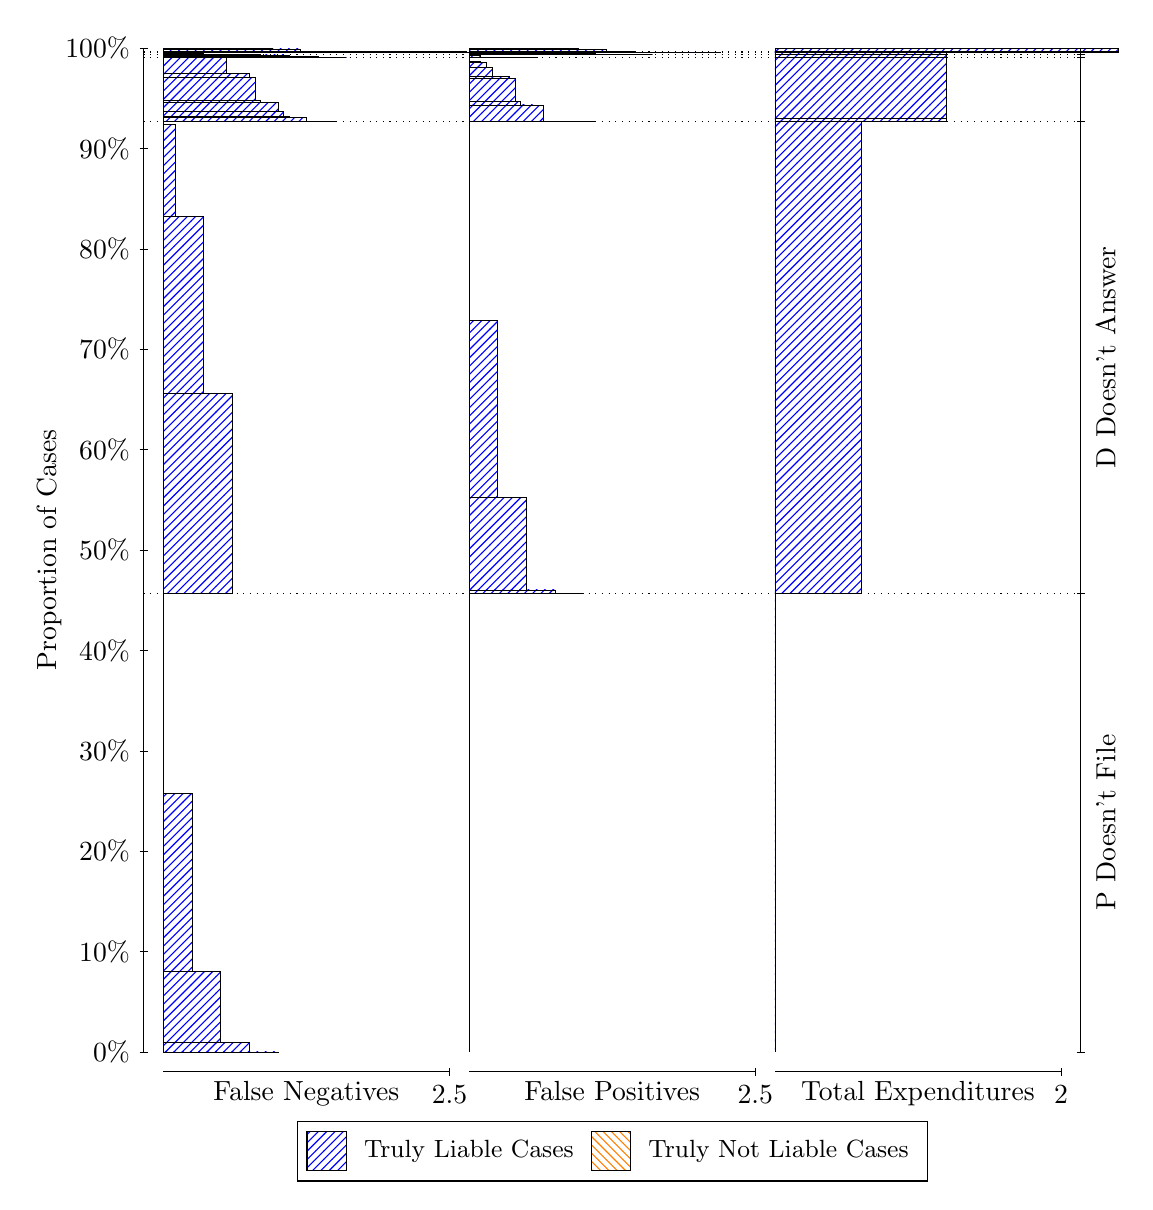
\begin{tikzpicture}
\draw[black, very thin] (1.5,1.75) -- (1.5,14.5);
\node[rotate=90, text=black, anchor=center] at (0.3, 8.125) {Proportion of Cases};
\draw[black, very thin] (1.45,1.75) -- (1.55,1.75);
\node[text=black, anchor=east] at (1.45, 1.75) {0\%};
\draw[black, very thin] (1.45,3.025) -- (1.55,3.025);
\node[text=black, anchor=east] at (1.45, 3.025) {10\%};
\draw[black, very thin] (1.45,4.3) -- (1.55,4.3);
\node[text=black, anchor=east] at (1.45, 4.3) {20\%};
\draw[black, very thin] (1.45,5.575) -- (1.55,5.575);
\node[text=black, anchor=east] at (1.45, 5.575) {30\%};
\draw[black, very thin] (1.45,6.85) -- (1.55,6.85);
\node[text=black, anchor=east] at (1.45, 6.85) {40\%};
\draw[black, very thin] (1.45,8.125) -- (1.55,8.125);
\node[text=black, anchor=east] at (1.45, 8.125) {50\%};
\draw[black, very thin] (1.45,9.4) -- (1.55,9.4);
\node[text=black, anchor=east] at (1.45, 9.4) {60\%};
\draw[black, very thin] (1.45,10.675) -- (1.55,10.675);
\node[text=black, anchor=east] at (1.45, 10.675) {70\%};
\draw[black, very thin] (1.45,11.95) -- (1.55,11.95);
\node[text=black, anchor=east] at (1.45, 11.95) {80\%};
\draw[black, very thin] (1.45,13.225) -- (1.55,13.225);
\node[text=black, anchor=east] at (1.45, 13.225) {90\%};
\draw[black, very thin] (1.45,14.5) -- (1.55,14.5);
\node[text=black, anchor=east] at (1.45, 14.5) {100\%};

\draw[black, very thin] (13.4,1.75) -- (13.4,14.5);
\draw[black, very thin] (13.35,1.75) -- (13.45,1.75);
\node[anchor=west] at (13.35, 1.75) {};
\draw[black, very thin] (13.35,7.5781) -- (13.45,7.5781);
\node[anchor=west] at (13.35, 7.5781) {};
\draw[black, very thin] (13.35,13.57) -- (13.45,13.57);
\node[anchor=west] at (13.35, 13.57) {};
\draw[black, very thin] (13.35,14.381) -- (13.45,14.381);
\node[anchor=west] at (13.35, 14.381) {};
\draw[black, very thin] (13.35,14.417) -- (13.45,14.417);
\node[anchor=west] at (13.35, 14.417) {};
\draw[black, very thin] (13.35,14.449) -- (13.45,14.449);
\node[anchor=west] at (13.35, 14.449) {};
\draw[black, very thin] (13.35,14.5) -- (13.45,14.5);
\node[anchor=west] at (13.35, 14.5) {};

\draw[black, very thin, pattern color=blue, pattern=north east lines] (1.75,1.75) rectangle (3.2033,1.7512);
\draw[black, very thin, pattern color=blue, pattern=north east lines] (1.75,1.7512) rectangle (2.84,1.8694);
\draw[black, very thin, pattern color=blue, pattern=north east lines] (1.75,1.8694) rectangle (2.4767,2.7714);
\draw[black, very thin, pattern color=blue, pattern=north east lines] (1.75,2.7714) rectangle (2.1133,5.031);
\draw[black, very thin, pattern color=orange, pattern=north west lines] (1.75,5.031) rectangle (1.75,5.031);
\draw[black, very thin, pattern color=blue, pattern=north east lines] (1.75,5.031) rectangle (1.75,7.5781);
\draw[black, very thin, pattern color=blue, pattern=north east lines] (1.75,7.5781) rectangle (2.622,10.11);
\draw[black, very thin, pattern color=blue, pattern=north east lines] (1.75,10.11) rectangle (2.2587,12.357);
\draw[black, very thin, pattern color=blue, pattern=north east lines] (1.75,12.357) rectangle (1.8953,13.53);
\draw[black, very thin, pattern color=orange, pattern=north west lines] (1.75,13.53) rectangle (1.75,13.53);
\draw[black, very thin, pattern color=blue, pattern=north east lines] (1.75,13.53) rectangle (1.75,13.57);
\draw[black, very thin, pattern color=blue, pattern=north east lines] (1.75,13.57) rectangle (3.93,13.571);
\draw[black, very thin, pattern color=blue, pattern=north east lines] (1.75,13.571) rectangle (3.6393,13.573);
\draw[black, very thin, pattern color=blue, pattern=north east lines] (1.75,13.573) rectangle (3.5667,13.622);
\draw[black, very thin, pattern color=blue, pattern=north east lines] (1.75,13.622) rectangle (3.3487,13.636);
\draw[black, very thin, pattern color=blue, pattern=north east lines] (1.75,13.636) rectangle (3.276,13.692);
\draw[black, very thin, pattern color=blue, pattern=north east lines] (1.75,13.692) rectangle (3.2033,13.81);
\draw[black, very thin, pattern color=blue, pattern=north east lines] (1.75,13.81) rectangle (2.9853,13.836);
\draw[black, very thin, pattern color=blue, pattern=north east lines] (1.75,13.836) rectangle (2.9127,14.127);
\draw[black, very thin, pattern color=blue, pattern=north east lines] (1.75,14.127) rectangle (2.84,14.175);
\draw[black, very thin, pattern color=blue, pattern=north east lines] (1.75,14.175) rectangle (2.622,14.179);
\draw[black, very thin, pattern color=blue, pattern=north east lines] (1.75,14.179) rectangle (2.5493,14.378);
\draw[black, very thin, pattern color=blue, pattern=north east lines] (1.75,14.378) rectangle (2.4767,14.379);
\draw[black, very thin, pattern color=blue, pattern=north east lines] (1.75,14.379) rectangle (2.2587,14.379);
\draw[black, very thin, pattern color=blue, pattern=north east lines] (1.75,14.379) rectangle (2.186,14.381);
\draw[black, very thin, pattern color=blue, pattern=north east lines] (1.75,14.381) rectangle (1.8953,14.381);
\draw[black, very thin, pattern color=orange, pattern=north west lines] (1.75,14.381) rectangle (1.75,14.381);
\draw[black, very thin, pattern color=blue, pattern=north east lines] (1.75,14.381) rectangle (4.0753,14.381);
\draw[black, very thin, pattern color=blue, pattern=north east lines] (1.75,14.381) rectangle (3.712,14.395);
\draw[black, very thin, pattern color=blue, pattern=north east lines] (1.75,14.395) rectangle (3.3487,14.414);
\draw[black, very thin, pattern color=blue, pattern=north east lines] (1.75,14.414) rectangle (2.9853,14.417);
\draw[black, very thin, pattern color=blue, pattern=north east lines] (1.75,14.417) rectangle (2.622,14.417);
\draw[black, very thin, pattern color=orange, pattern=north west lines] (1.75,14.417) rectangle (1.75,14.417);
\draw[black, very thin, pattern color=blue, pattern=north east lines] (1.75,14.417) rectangle (2.622,14.417);
\draw[black, very thin, pattern color=blue, pattern=north east lines] (1.75,14.417) rectangle (2.2587,14.436);
\draw[black, very thin, pattern color=blue, pattern=north east lines] (1.75,14.436) rectangle (1.8953,14.449);
\draw[black, very thin, pattern color=orange, pattern=north west lines] (1.75,14.449) rectangle (1.75,14.449);
\draw[black, very thin, pattern color=blue, pattern=north east lines] (1.75,14.449) rectangle (1.75,14.449);
\draw[black, very thin, pattern color=blue, pattern=north east lines] (1.75,14.449) rectangle (6.6913,14.449);
\draw[black, very thin, pattern color=blue, pattern=north east lines] (1.75,14.449) rectangle (6.328,14.449);
\draw[black, very thin, pattern color=blue, pattern=north east lines] (1.75,14.449) rectangle (5.9647,14.449);
\draw[black, very thin, pattern color=blue, pattern=north east lines] (1.75,14.449) rectangle (5.6013,14.453);
\draw[black, very thin, pattern color=blue, pattern=north east lines] (1.75,14.453) rectangle (5.238,14.453);
\draw[black, very thin, pattern color=blue, pattern=north east lines] (1.75,14.453) rectangle (4.8747,14.453);
\draw[black, very thin, pattern color=blue, pattern=north east lines] (1.75,14.453) rectangle (4.584,14.453);
\draw[black, very thin, pattern color=blue, pattern=north east lines] (1.75,14.453) rectangle (4.2207,14.454);
\draw[black, very thin, pattern color=blue, pattern=north east lines] (1.75,14.454) rectangle (3.8573,14.462);
\draw[black, very thin, pattern color=blue, pattern=north east lines] (1.75,14.462) rectangle (3.494,14.488);
\draw[black, very thin, pattern color=blue, pattern=north east lines] (1.75,14.488) rectangle (3.1307,14.499);
\draw[black, very thin, pattern color=blue, pattern=north east lines] (1.75,14.499) rectangle (2.7673,14.5);
\draw[black, very thin, pattern color=blue, pattern=north east lines] (1.75,14.5) rectangle (2.404,14.5);
\draw[black, very thin, pattern color=blue, pattern=north east lines] (1.75,14.5) rectangle (2.0407,14.5);
\draw[black, very thin, pattern color=orange, pattern=north west lines] (1.75,14.5) rectangle (1.75,14.5);
\draw[black, very thin, pattern color=orange, pattern=north west lines] (5.6333,1.75) rectangle (5.6333,1.75);
\draw[black, very thin, pattern color=blue, pattern=north east lines] (5.6333,1.75) rectangle (5.6333,7.5781);
\draw[black, very thin, pattern color=orange, pattern=north west lines] (5.6333,7.5781) rectangle (7.0867,7.5781);
\draw[black, very thin, pattern color=blue, pattern=north east lines] (5.6333,7.5781) rectangle (7.0867,7.5781);
\draw[black, very thin, pattern color=blue, pattern=north east lines] (5.6333,7.5781) rectangle (6.7233,7.6183);
\draw[black, very thin, pattern color=blue, pattern=north east lines] (5.6333,7.6183) rectangle (6.36,8.7914);
\draw[black, very thin, pattern color=blue, pattern=north east lines] (5.6333,8.7914) rectangle (5.9967,11.039);
\draw[black, very thin, pattern color=blue, pattern=north east lines] (5.6333,11.039) rectangle (5.6333,13.57);
\draw[black, very thin, pattern color=orange, pattern=north west lines] (5.6333,13.57) rectangle (7.232,13.57);
\draw[black, very thin, pattern color=blue, pattern=north east lines] (5.6333,13.57) rectangle (7.232,13.57);
\draw[black, very thin, pattern color=orange, pattern=north west lines] (5.6333,13.57) rectangle (6.9413,13.57);
\draw[black, very thin, pattern color=blue, pattern=north east lines] (5.6333,13.57) rectangle (6.9413,13.573);
\draw[black, very thin, pattern color=blue, pattern=north east lines] (5.6333,13.573) rectangle (6.8687,13.573);
\draw[black, very thin, pattern color=orange, pattern=north west lines] (5.6333,13.573) rectangle (6.6507,13.573);
\draw[black, very thin, pattern color=blue, pattern=north east lines] (5.6333,13.573) rectangle (6.6507,13.573);
\draw[black, very thin, pattern color=blue, pattern=north east lines] (5.6333,13.573) rectangle (6.578,13.772);
\draw[black, very thin, pattern color=blue, pattern=north east lines] (5.6333,13.772) rectangle (6.5053,13.777);
\draw[black, very thin, pattern color=blue, pattern=north east lines] (5.6333,13.777) rectangle (6.2873,13.825);
\draw[black, very thin, pattern color=blue, pattern=north east lines] (5.6333,13.825) rectangle (6.2147,14.116);
\draw[black, very thin, pattern color=blue, pattern=north east lines] (5.6333,14.116) rectangle (6.142,14.141);
\draw[black, very thin, pattern color=blue, pattern=north east lines] (5.6333,14.141) rectangle (5.924,14.259);
\draw[black, very thin, pattern color=blue, pattern=north east lines] (5.6333,14.259) rectangle (5.8513,14.316);
\draw[black, very thin, pattern color=blue, pattern=north east lines] (5.6333,14.316) rectangle (5.7787,14.329);
\draw[black, very thin, pattern color=blue, pattern=north east lines] (5.6333,14.329) rectangle (5.6333,14.381);
\draw[black, very thin, pattern color=orange, pattern=north west lines] (5.6333,14.381) rectangle (6.5053,14.381);
\draw[black, very thin, pattern color=blue, pattern=north east lines] (5.6333,14.381) rectangle (6.5053,14.381);
\draw[black, very thin, pattern color=blue, pattern=north east lines] (5.6333,14.381) rectangle (6.142,14.383);
\draw[black, very thin, pattern color=blue, pattern=north east lines] (5.6333,14.383) rectangle (5.7787,14.403);
\draw[black, very thin, pattern color=blue, pattern=north east lines] (5.6333,14.403) rectangle (5.6333,14.417);
\draw[black, very thin, pattern color=orange, pattern=north west lines] (5.6333,14.417) rectangle (7.9587,14.417);
\draw[black, very thin, pattern color=blue, pattern=north east lines] (5.6333,14.417) rectangle (7.9587,14.417);
\draw[black, very thin, pattern color=blue, pattern=north east lines] (5.6333,14.417) rectangle (7.5953,14.417);
\draw[black, very thin, pattern color=blue, pattern=north east lines] (5.6333,14.417) rectangle (7.232,14.43);
\draw[black, very thin, pattern color=blue, pattern=north east lines] (5.6333,14.43) rectangle (6.8687,14.448);
\draw[black, very thin, pattern color=blue, pattern=north east lines] (5.6333,14.448) rectangle (6.5053,14.449);
\draw[black, very thin, pattern color=orange, pattern=north west lines] (5.6333,14.449) rectangle (8.8307,14.449);
\draw[black, very thin, pattern color=blue, pattern=north east lines] (5.6333,14.449) rectangle (8.8307,14.449);
\draw[black, very thin, pattern color=blue, pattern=north east lines] (5.6333,14.449) rectangle (8.4673,14.449);
\draw[black, very thin, pattern color=orange, pattern=north west lines] (5.6333,14.449) rectangle (8.4673,14.449);
\draw[black, very thin, pattern color=blue, pattern=north east lines] (5.6333,14.449) rectangle (8.4673,14.449);
\draw[black, very thin, pattern color=blue, pattern=north east lines] (5.6333,14.449) rectangle (8.104,14.449);
\draw[black, very thin, pattern color=orange, pattern=north west lines] (5.6333,14.449) rectangle (8.104,14.449);
\draw[black, very thin, pattern color=blue, pattern=north east lines] (5.6333,14.449) rectangle (8.104,14.449);
\draw[black, very thin, pattern color=blue, pattern=north east lines] (5.6333,14.449) rectangle (7.7407,14.454);
\draw[black, very thin, pattern color=orange, pattern=north west lines] (5.6333,14.454) rectangle (7.7407,14.454);
\draw[black, very thin, pattern color=blue, pattern=north east lines] (5.6333,14.454) rectangle (7.7407,14.461);
\draw[black, very thin, pattern color=blue, pattern=north east lines] (5.6333,14.461) rectangle (7.3773,14.462);
\draw[black, very thin, pattern color=blue, pattern=north east lines] (5.6333,14.462) rectangle (7.3773,14.487);
\draw[black, very thin, pattern color=blue, pattern=north east lines] (5.6333,14.487) rectangle (7.014,14.495);
\draw[black, very thin, pattern color=blue, pattern=north east lines] (5.6333,14.495) rectangle (6.6507,14.496);
\draw[black, very thin, pattern color=blue, pattern=north east lines] (5.6333,14.496) rectangle (6.2873,14.496);
\draw[black, very thin, pattern color=orange, pattern=north west lines] (5.6333,14.496) rectangle (5.9967,14.496);
\draw[black, very thin, pattern color=blue, pattern=north east lines] (5.6333,14.496) rectangle (5.9967,14.496);
\draw[black, very thin, pattern color=orange, pattern=north west lines] (5.6333,14.496) rectangle (5.6333,14.496);
\draw[black, very thin, pattern color=blue, pattern=north east lines] (5.6333,14.496) rectangle (5.6333,14.5);
\draw[black, very thin, pattern color=orange, pattern=north west lines] (9.5167,1.75) rectangle (9.5167,1.75);
\draw[black, very thin, pattern color=blue, pattern=north east lines] (9.5167,1.75) rectangle (9.5167,7.5781);
\draw[black, very thin, pattern color=orange, pattern=north west lines] (9.5167,7.5781) rectangle (10.607,7.5781);
\draw[black, very thin, pattern color=blue, pattern=north east lines] (9.5167,7.5781) rectangle (10.607,13.57);
\draw[black, very thin, pattern color=orange, pattern=north west lines] (9.5167,13.57) rectangle (11.697,13.57);
\draw[black, very thin, pattern color=blue, pattern=north east lines] (9.5167,13.57) rectangle (11.697,13.614);
\draw[black, very thin, pattern color=orange, pattern=north west lines] (9.5167,13.614) rectangle (11.697,13.614);
\draw[black, very thin, pattern color=blue, pattern=north east lines] (9.5167,13.614) rectangle (11.697,14.381);
\draw[black, very thin, pattern color=orange, pattern=north west lines] (9.5167,14.381) rectangle (11.697,14.381);
\draw[black, very thin, pattern color=blue, pattern=north east lines] (9.5167,14.381) rectangle (11.697,14.417);
\draw[black, very thin, pattern color=orange, pattern=north west lines] (9.5167,14.417) rectangle (11.697,14.417);
\draw[black, very thin, pattern color=blue, pattern=north east lines] (9.5167,14.417) rectangle (11.697,14.449);
\draw[black, very thin, pattern color=orange, pattern=north west lines] (9.5167,14.449) rectangle (13.877,14.449);
\draw[black, very thin, pattern color=blue, pattern=north east lines] (9.5167,14.449) rectangle (13.877,14.455);
\draw[black, very thin, pattern color=orange, pattern=north west lines] (9.5167,14.455) rectangle (13.877,14.455);
\draw[black, very thin, pattern color=blue, pattern=north east lines] (9.5167,14.455) rectangle (13.877,14.5);
\draw[black, dotted] (1.5,7.5781) -- (13.4,7.5781);
\draw[black, dotted] (1.5,13.57) -- (13.4,13.57);
\draw[black, dotted] (1.5,14.381) -- (13.4,14.381);
\draw[black, dotted] (1.5,14.417) -- (13.4,14.417);
\draw[black, dotted] (1.5,14.449) -- (13.4,14.449);
\draw[black, very thin] (1.75,1.5) -- (5.3833,1.5);
\node[text=black, anchor=north] at (3.5667, 1.5) {False Negatives};
\draw[black, very thin] (5.3833,1.45) -- (5.3833,1.55);
\node[text=black, anchor=north] at (5.3833, 1.45) {2.5};

\draw[black, very thin] (5.6333,1.5) -- (9.2667,1.5);
\node[text=black, anchor=north] at (7.45, 1.5) {False Positives};
\draw[black, very thin] (9.2667,1.45) -- (9.2667,1.55);
\node[text=black, anchor=north] at (9.2667, 1.45) {2.5};

\draw[black, very thin] (9.5167,1.5) -- (13.15,1.5);
\node[text=black, anchor=north] at (11.333, 1.5) {Total Expenditures};
\draw[black, very thin] (13.15,1.45) -- (13.15,1.55);
\node[text=black, anchor=north] at (13.15, 1.45) {2};

\node[text=black, centered, rotate=90] at (13.72, 4.6641) {P Doesn't File};
\node[text=black, centered, rotate=90] at (13.72, 10.574) {D Doesn't Answer};





\draw (7.449999999999999,1.5) node[draw=none] (baseCoordinate) {};
\begin{scope}[align=center]
        \matrix[scale=0.5, draw=black, below=0.5cm of baseCoordinate, nodes={draw}, column sep=0.1cm]{
            \node[rectangle, draw, minimum width=0.5cm, minimum height=0.5cm, pattern color=blue, pattern=north east lines] {}; &
            \node[draw=none, font=\small, text=black] (B) {Truly Liable Cases}; &
            \node[rectangle, draw, minimum width=0.5cm, minimum height=0.5cm, pattern color=orange, pattern=north west lines] {}; &
            \node[draw=none, font=\small, text=black] (B) {Truly Not Liable Cases}; \\
            };
\end{scope}

\end{tikzpicture}
\end{document}